\documentclass[11pt]{article} % use larger type; default would be 10pt

\usepackage{graphicx} % support the \includegraphics command and options
\usepackage[margin=1.0in]{geometry}
\usepackage{amssymb}
\usepackage{amsmath}

\title{\textsc{The Partitioned Element Method} \\ \textbf{Supplementary Notes}}
\author{B. Giffin}
\date{}

\begin{document}
\maketitle

\section{Definitions}
The following set of definitions are directed towards the PEM face minimum problem (as a representative example of the various tope-specific minimum problems of the PEM).
\begin{figure} [!ht]
	\centering
	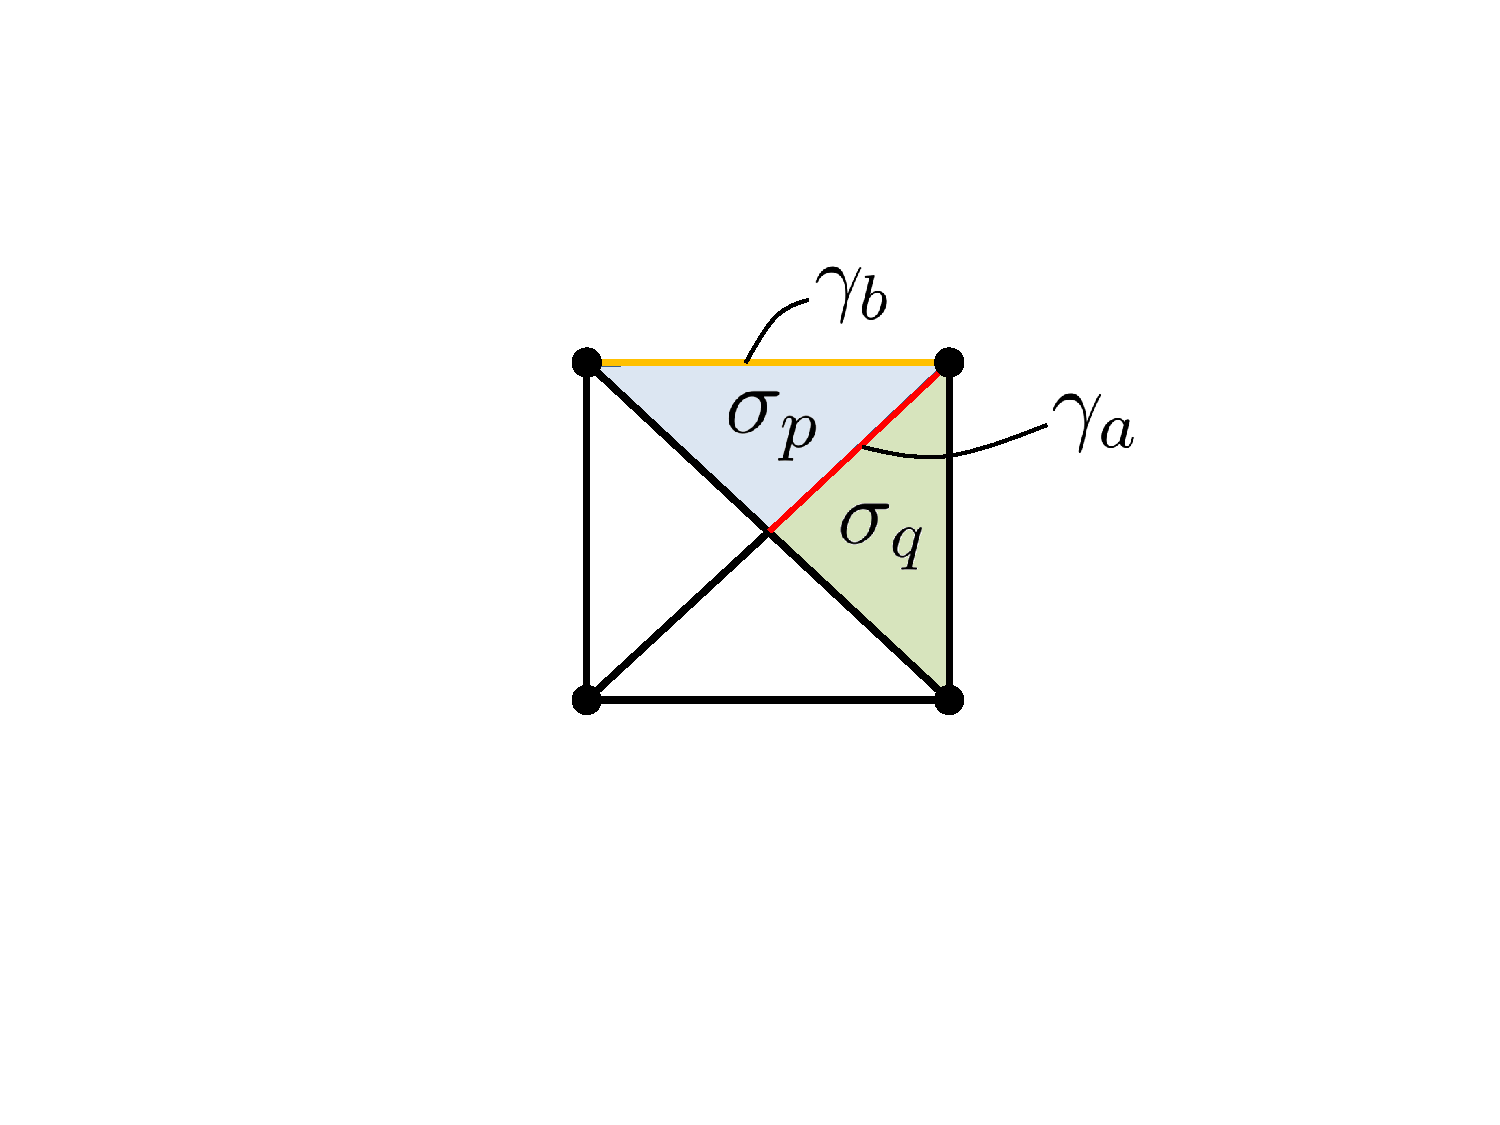
\includegraphics[width = 2.8in,trim=170 190 170 120,clip=true]{facetMinImage.pdf}
	\caption{A representative face of interest.}
	\label{fig:facetMin}
\end{figure}
\begin{itemize}
	\item[$\sigma_p$:] A facet on the current face of interest.
	\item[$| \sigma_p |$:] The area of facet $\sigma_p$.
	\item[$c_p$, $\mathbf{g}_p$:] The unknown coefficients that describe the variation of a particular nodal shape function within facet $p$:
	\begin{equation}
		\varphi_p (\mathbf{x}) = c_p + (\mathbf{x} - \mathbf{x}_p) \cdot \mathbf{g}_p
	\end{equation}
	\item[$\mathbf{n}_p$:] The surface normal of facet $p$.
	\item[$\mathbf{x}_p$:] An arbitrarily chosen reference position on facet $p$.
	\item[$\mathcal{L}$:] The set of all ``interior'' segments belonging to the current face.
	\item[$\mathcal{B}$:] The set of all ``boundary'' segments belonging to the current face.
	\item[$\gamma_a$:] An ``interior'' segment, such that $a \in \mathcal{L}$; one that borders two facets: $\sigma_p$ and $\sigma_q$.
	\item[$\gamma_b$:] A ``boundary'' segment, such that $b \in \mathcal{B}$; one that borders a single facet: $\sigma_p$.
	\item[$\bar{c}_b$, $\bar{\mathbf{g}}_b$:] The known coefficients that describe the variation of a particular nodal shape function within segment $b$:
	\begin{equation}
		\varphi_b (\mathbf{x}) = \bar{c}_b + (\mathbf{x} - \mathbf{x}_b) \cdot \bar{\mathbf{g}}_b
	\end{equation}
	\item[$\mathbf{x}_b$:] An arbitrarily chosen reference position on segment $b$.
	\item[$| \gamma_a |$:] The length of segment $\gamma_a$ (similarly for $| \gamma_b |$).
	\item[$\mathbf{P}^c_a$:] A segment subspace projection operator which maps arbitrary vectors in $\mathbb{R}^3$ to the one-dimensional manifold associated with segment $\gamma_a$. If the tangent space to this manifold is spanned by a single vector $\lambda_a \in \mathbb{R}^3$, then we can determine $\mathbf{P}^c_a$ via:
	\begin{equation}
		\mathbf{P}^c_a = \lambda_a \otimes \lambda_a
	\end{equation}
	\item[$\mathbf{P}_a$:] A complementary subspace projection operator which maps arbitrary vectors in $\mathbb{R}^3$ to the complement of the subspace associated with $\mathbf{P}^c_a$, obtained via:
	\begin{equation}
		\mathbf{P}_a = \mathbf{1} - \mathbf{P}^c_a
	\end{equation}
	\item[$\varepsilon$:] A scalar-valued measure of the jump in value of a given shape function on interior segments:
	\begin{equation}
		\varepsilon = \varphi_p (\mathbf{x}) - \varphi_q (\mathbf{x})
	\end{equation}
	\begin{equation}
		\varepsilon = c_p + (\mathbf{x} - \mathbf{x}_p) \cdot \mathbf{g}_p - c_q - (\mathbf{x} - \mathbf{x}_q) \cdot \mathbf{g}_q
	\end{equation}
	on boundary segments:
	\begin{equation}
		\varepsilon = \varphi_p (\mathbf{x}) - \varphi_b (\mathbf{x})
	\end{equation}
	\begin{equation}
		\varepsilon = c_p + (\mathbf{x} - \mathbf{x}_p) \cdot \mathbf{g}_p - \bar{c}_b - (\mathbf{x} - \mathbf{x}_b) \cdot \bar{\mathbf{g}}_b
	\end{equation}
	\item[$\Delta$:] A vector-valued measure of the jump in normal derivative of a given shape function, evaluated on an interior segment $\gamma_a$ bordering facets $\sigma_p$ and $\sigma_q$:
	\begin{equation}
		\Delta =\mathbf{P}^c_a ( \nabla \varphi_p (\mathbf{x}) - \nabla \varphi_q (\mathbf{x}) )
	\end{equation}
	\begin{equation}
		\Delta =\mathbf{P}^c_a ( \mathbf{g}_p - \mathbf{g}_q )
	\end{equation}
	\item[$\beta$:] An adjustable parameter, such that $\beta \in (0, 1)$. If $\beta = 0$, $\mathcal{F}$ only penalizes jumps in the normal derivative of the shape function between facets (evaluated on \textit{interior} segments). This effects ``smoothness'' (approaching $C^1$ continuity) of the resulting shape functions. If $\beta = 1$, $\mathcal{F}$ only penalizes jumps in the value of the shape function between facets (evaluated on \textit{interior} segments). This effects $C^0$ continuity of the resulting shape functions (on the interior of the face).
	\item[$\alpha$:] Yet another adjustable parameter such that $\alpha \in (0, 1)$. If $\alpha = 1$, $\mathcal{F}$ will penalize jumps in the value of the shape function between facets and the boundary of the face (evaluated on \textit{boundary} segments). This effects $C^0$ continuity of the resulting shape functions (on the boundary of the face), with no regard for continuity or smoothness across interior segments. If $\alpha = 0$, $\mathcal{F}$ will be expressed only by the relevant $\beta$ terms, meaning there is no penalization to effect continuity with the boundary segments.
	\item[$\mathcal{F}$:] The quadratic functional for a face that is to be minimized with respect to $c_p$ and $\mathbf{g}_p$ for all facets $p$:
	\begin{eqnarray}
	\mathcal{F} = (1-\alpha) \left[ (1-\beta) \sum_{a \in \mathcal{L}} | \gamma_a | \int_{\gamma_a} \frac{1}{2} \Delta \cdot \Delta d \xi + \beta \sum_{a \in \mathcal{L}} \frac{1}{| \gamma_a |} \int_{\gamma_a} \frac{1}{2} \varepsilon^2 d \xi \right] \nonumber \\ + \alpha \sum_{b \in \mathcal{B}} \frac{1}{| \gamma_b |} \int_{\gamma_b} \frac{1}{2} \varepsilon^2 d \xi
\end{eqnarray}
\end{itemize}

\section{Quasi-linear PEM (Face) Shape Functions}

Now that we have taken care of the relevant definitions, we may elaborate on the minimization procedure. Ultimately, we seek the unknown coefficients $c_p$ and $\mathbf{g}_p$ for all facets $p$ of a given face. These are obtained via
\begin{equation}
	\min_{c_p, \, \mathbf{g}_p} \mathcal{F} \, \, \forall p
\end{equation}
It proves convenient to look at the minimization associated with only one particular interior segment $\gamma_a$:
\begin{equation}
	\mathcal{F}^a = (1-\alpha) \left[ (1-\beta) | \gamma_a | \int_{\gamma_a} \frac{1}{2} \Delta \cdot \Delta d \xi + \beta \frac{1}{| \gamma_a |} \int_{\gamma_a} \frac{1}{2} \varepsilon^2 d \xi \right]
\end{equation}
\begin{equation}
	\frac{\partial \mathcal{F}^a}{\partial c_p} = 0; \qquad \frac{\partial \mathcal{F}^a}{\partial \mathbf{g}_p} = \mathbf{0}
\end{equation}
\begin{equation}
	\frac{\partial \mathcal{F}^a}{\partial c_q} = 0; \qquad \frac{\partial \mathcal{F}^a}{\partial \mathbf{g}_q} = \mathbf{0}
\end{equation}
and one particular boundary segment $\gamma_b$:
\begin{equation}
	\mathcal{F}^b = \alpha \frac{1}{| \gamma_b |} \int_{\gamma_b} \frac{1}{2} \varepsilon^2 d \xi
\end{equation}
\begin{equation}
	\frac{\partial \mathcal{F}^b}{\partial c_p} = 0; \qquad \frac{\partial \mathcal{F}^b}{\partial \mathbf{g}_p} = \mathbf{0}
\end{equation}

For the interior segment:
\begin{equation}
	\frac{\partial \mathcal{F}^a}{\partial c_p} = (1-\alpha) \left[ (1-\beta) | \gamma_a | \int_{\gamma_a} \Delta \cdot \frac{\partial \Delta}{\partial c_p} d \xi + \beta \frac{1}{| \gamma_a |} \int_{\gamma_a} \varepsilon \frac{\partial \varepsilon}{\partial c_p} d \xi \right]
\end{equation}
\begin{equation}
	\frac{\partial \mathcal{F}^a}{\partial \mathbf{g}_p} = (1-\alpha) \left[ (1-\beta) | \gamma_a | \int_{\gamma_a} \Delta \cdot \frac{\partial \Delta}{\partial \mathbf{g}_p} d \xi + \beta \frac{1}{| \gamma_a |} \int_{\gamma_a} \varepsilon \frac{\partial \varepsilon}{\partial \mathbf{g}_p} d \xi \right]
\end{equation}
\begin{equation}
	\frac{\partial \mathcal{F}^a}{\partial c_q} = (1-\alpha) \left[ (1-\beta) | \gamma_a | \int_{\gamma_a} \Delta \cdot \frac{\partial \Delta}{\partial c_q} d \xi + \beta \frac{1}{| \gamma_a |} \int_{\gamma_a} \varepsilon \frac{\partial \varepsilon}{\partial c_q} d \xi \right]
\end{equation}
\begin{equation}
	\frac{\partial \mathcal{F}^a}{\partial \mathbf{g}_q} = (1-\alpha) \left[ (1-\beta) | \gamma_a | \int_{\gamma_a} \Delta \cdot \frac{\partial \Delta}{\partial \mathbf{g}_q} d \xi + \beta \frac{1}{| \gamma_a |} \int_{\gamma_a} \varepsilon \frac{\partial \varepsilon}{\partial \mathbf{g}_q} d \xi \right]
\end{equation}
Examining terms of interest, we find
\begin{equation}
	\frac{\partial \Delta}{\partial c_p} = \frac{\partial \Delta}{\partial c_q} = 0
\end{equation}
\begin{equation}
	\frac{\partial \varepsilon}{\partial c_p} = - \frac{\partial \varepsilon}{\partial c_q} = 1
\end{equation}
\begin{equation}
	\frac{\partial \Delta}{\partial \mathbf{g}_p} = - \frac{\partial \Delta}{\partial \mathbf{g}_q} = \mathbf{P}_a
\end{equation}
\begin{equation}
	\frac{\partial \varepsilon}{\partial \mathbf{g}_p} = (\mathbf{x} - \mathbf{x}_p), \quad \frac{\partial \varepsilon}{\partial \mathbf{g}_q} = -(\mathbf{x} - \mathbf{x}_q)
\end{equation}
Making the appropriate substitutions,
\begin{equation}
	\frac{\partial \mathcal{F}^a}{\partial c_p} = (1-\alpha) \left[ \beta \frac{1}{| \gamma_a |} \int_{\gamma_a} \left[ c_p + (\mathbf{x} - \mathbf{x}_p) \cdot \mathbf{g}_p - c_q - (\mathbf{x} - \mathbf{x}_q) \cdot \mathbf{g}_q \right] d \xi \right]
\end{equation}
\begin{equation}
	\frac{\partial \mathcal{F}^a}{\partial c_q} = (1-\alpha) \left[ \beta \frac{1}{| \gamma_a |} \int_{\gamma_a} \left[ -c_p - (\mathbf{x} - \mathbf{x}_p) \cdot \mathbf{g}_p + c_q + (\mathbf{x} - \mathbf{x}_q) \cdot \mathbf{g}_q \right] d \xi \right]
\end{equation}
\begin{eqnarray}
	\frac{\partial \mathcal{F}^a}{\partial \mathbf{g}_p} = (1-\alpha) \left[ (1-\beta) | \gamma_a | \int_{\gamma_a} \mathbf{P}_a (\mathbf{g}_p - \mathbf{g}_q ) \, d \xi \right. \nonumber \\ + \left. \beta \frac{1}{| \gamma_a |} \int_{\gamma_a} \left[ c_p + (\mathbf{x} - \mathbf{x}_p) \cdot \mathbf{g}_p - c_q - (\mathbf{x} - \mathbf{x}_q) \cdot \mathbf{g}_q \right] (\mathbf{x} - \mathbf{x}_p) \, d \xi \right]
\end{eqnarray}
\begin{eqnarray}
	\frac{\partial \mathcal{F}^a}{\partial \mathbf{g}_q} = (1-\alpha) \left[ (1-\beta) | \gamma_a | \int_{\gamma_a} \mathbf{P}_a (- \mathbf{g}_p + \mathbf{g}_q ) \, d \xi \right. \nonumber \\ + \left. \beta \frac{1}{| \gamma_a |} \int_{\gamma_a} \left[ -c_p - (\mathbf{x} - \mathbf{x}_p) \cdot \mathbf{g}_p + c_q + (\mathbf{x} - \mathbf{x}_q) \cdot \mathbf{g}_q \right] (\mathbf{x} - \mathbf{x}_q) d \xi \right]
\end{eqnarray}
If we define the following terms:
\begin{equation}
	k_{cc} = (1-\alpha) \beta \frac{1}{| \gamma_a |} \int_{\gamma_a} d \xi \quad (1 \times 1)
\end{equation}
\begin{equation}
	\mathbf{k}_{cg}^{(q)} = (1-\alpha) \beta \frac{1}{| \gamma_a |} \int_{\gamma_a} (\mathbf{x} - \mathbf{x}_q) \, d \xi \quad (1 \times 3)
\end{equation}
\begin{equation}
	\mathbf{k}_{gc}^{(p)} = (1-\alpha) \beta \frac{1}{| \gamma_a |} \int_{\gamma_a} (\mathbf{x} - \mathbf{x}_p) d \xi \quad (3 \times 1)
\end{equation}
\begin{eqnarray}
	\mathbf{k}_{gg}^{(p,q)} = (1-\alpha) \left[ \beta \frac{1}{| \gamma_a |} \int_{\gamma_a} (\mathbf{x} - \mathbf{x}_p) \otimes (\mathbf{x} - \mathbf{x}_q) \, d \xi + (1-\beta) | \gamma_a | \int_{\gamma_a} \mathbf{P}_a \, d \xi \right] \quad (3 \times 3)
\end{eqnarray}
and if we further define:
\begin{equation}
	\mathbf{K}_{pq}^{(a)} = \left[ \begin{array}{cc} k_{cc} & \mathbf{k}_{cg}^{(q)} \\ \mathbf{k}_{gc}^{(p)} & \mathbf{k}_{gg}^{(p,q)} \end{array} \right] \quad (4 \times 4)
\end{equation}
\begin{equation}
	\mathbf{u}_p = \left\{ \begin{array}{c} c_p \\ \mathbf{g}_p \end{array} \right\} \quad (4 \times 1)
\end{equation}
then we may recast the local minimization for segment $a$ in the form of a local $8\times8$ contribution to the global minimization problem:
\begin{equation}
	\left[ \begin{array}{cc} \mathbf{K}_{pp}^{(a)} & -\mathbf{K}_{pq}^{(a)} \\ -\mathbf{K}_{qp}^{(a)} & \mathbf{K}_{qq}^{(a)} \end{array} \right] \left\{ \begin{array}{c} \mathbf{u}_p \\ \mathbf{u}_q \end{array} \right\} = \left\{ \begin{array}{c} \mathbf{0} \\ \mathbf{0} \end{array} \right\}
\end{equation}

We may proceed in a similar manner to determine a local contribution from the boundary segment:
\begin{equation}
	\frac{\partial \mathcal{F}^b}{\partial c_p} = \alpha \frac{1}{| \gamma_b |} \int_{\gamma_b} \varepsilon \frac{\partial \varepsilon}{\partial c_p} d \xi
\end{equation}
\begin{equation}
	\frac{\partial \mathcal{F}^b}{\partial \mathbf{g}_p} = \alpha \frac{1}{| \gamma_b |} \int_{\gamma_b} \varepsilon \frac{\partial \varepsilon}{\partial \mathbf{g}_p} d \xi
\end{equation}
We recall
\begin{equation}
	\frac{\partial \varepsilon}{\partial c_p} = 1, \quad \frac{\partial \varepsilon}{\partial \mathbf{g}_p} = (\mathbf{x} - \mathbf{x}_p)
\end{equation}
Making the appropriate substitutions,
\begin{equation}
	\frac{\partial \mathcal{F}^b}{\partial c_p} = \alpha \frac{1}{| \gamma_b |} \int_{\gamma_b} \left[ c_p + (\mathbf{x} - \mathbf{x}_p) \cdot \mathbf{g}_p - \bar{c}_b - (\mathbf{x} - \mathbf{x}_b) \cdot \bar{\mathbf{g}}_b \right] d \xi
\end{equation}
\begin{eqnarray}
	\frac{\partial \mathcal{F}^b}{\partial \mathbf{g}_p} = \alpha \frac{1}{| \gamma_b |} \int_{\gamma_b} \left[ c_p + (\mathbf{x} - \mathbf{x}_p) \cdot \mathbf{g}_p - \bar{c}_b - (\mathbf{x} - \mathbf{x}_b) \cdot \bar{\mathbf{g}}_b \right] (\mathbf{x} - \mathbf{x}_p) d \xi
\end{eqnarray}
If we define the following terms:
\begin{equation}
	\bar{k}_{cc} = \alpha \frac{1}{| \gamma_b |} \int_{\gamma_b} d \xi \quad (1 \times 1)
\end{equation}
\begin{equation}
	\bar{\mathbf{k}}_{cg}^{(b)} = \alpha \frac{1}{| \gamma_b |} \int_{\gamma_b} (\mathbf{x} - \mathbf{x}_b) d \xi \quad (1 \times 3)
\end{equation}
\begin{equation}
	\bar{\mathbf{k}}_{gc}^{(p)} = \alpha \frac{1}{| \gamma_b |} \int_{\gamma_b} (\mathbf{x} - \mathbf{x}_p) d \xi \quad (3 \times 1)
\end{equation}
\begin{eqnarray}
	\bar{\mathbf{k}}_{gg}^{(p,b)} = \alpha \frac{1}{| \gamma_b |} \int_{\gamma_b} (\mathbf{x} - \mathbf{x}_p) \otimes (\mathbf{x} - \mathbf{x}_b) d \xi \quad (3 \times 3)
\end{eqnarray}
and if we further define:
\begin{equation}
	\bar{\mathbf{K}}_{pb}^{(b)} = \left[ \begin{array}{cc} \bar{k}_{cc} & \bar{\mathbf{k}}_{cg}^{(b)} \\ \bar{\mathbf{k}}_{gc}^{(p)} & \bar{\mathbf{k}}_{gg}^{(p,b)} \end{array} \right] \quad (4 \times 4)
\end{equation}
\begin{equation}
	\bar{\mathbf{u}}_b = \left\{ \begin{array}{c} \bar{c}_b \\ \bar{\mathbf{g}}_b \end{array} \right\} \quad (4 \times 1)
\end{equation}
then we may recast the local minimization for segment $b$ in the form of local $4\times4$ contributions to the global minimization problem:
\begin{equation}
	\bar{\mathbf{K}}_{pp}^{(b)} \mathbf{u}_p = \bar{\mathbf{K}}_{pb}^{(b)} \bar{\mathbf{u}}_b
\end{equation}

\newpage

\section{Integration of Polynomial Expressions on Arbitrary Polytopes}

Suppose we wish to integrate a polynomial expression $P^{(p)}(\mathbf{x})$ of degree $p$
\begin{equation}
	P^{(p)}(\mathbf{x}) = \sum_{r=0}^{p} a_r \mathbf{x}^{\otimes r}
\end{equation}
over an arbitrary closed $n$-polytope $\Omega_q \subset \mathcal{V}$ ($\mathcal{V}$ being an isometry of $\mathbb{R}^n$), which itself is embedded in $\mathbb{R}^d$ (such that $\mathbf{x} \in \mathbb{R}^d$). We identify $\mathbf{x}^{\otimes r}$ as a tensor of rank $r$ (e.g. $\mathbf{x}^{\otimes 2} = \mathbf{x} \otimes \mathbf{x}$). We are interested in computing
\begin{equation}
	\int_{\Omega_q} P^{(p)}(\mathbf{x}) d \Omega = \sum_{r=0}^{p} a_r \int_{\Omega_q} \mathbf{x}^{\otimes r} d \Omega,
\end{equation}
meaning we must be able to integrate $\int_{\Omega_q} \mathbf{x}^{\otimes r} d \Omega \, \, \forall r$. Let us suppose that $\mathbf{x}$ may be written as $\mathbf{x} = \mathbf{x}_q + \hat{\mathbf{x}}$, where $\mathbf{x}_q \in \mathbb{R}^d$ is some fixed reference position on the $n$-polytope, and $\hat{\mathbf{x}} \in \mathcal{V}$ is variable. Thus,
\begin{equation}
	\int_{\Omega_q} \mathbf{x}^{\otimes r} d \Omega = \int_{\Omega_q} (\mathbf{x}_q + \hat{\mathbf{x}})^{\otimes r} d \Omega = \sum_{k = 0}^r \binom{r}{k} \, \mbox{Sym}
\bigg( \mathbf{x}_q^{\otimes (r-k)} \otimes \int_{\Omega_q} \hat{\mathbf{x}}^{\otimes k} d \Omega \bigg) ,
\end{equation}
where $\mbox{Sym} ( \mathbf{T} )$ denotes the symmetric part of tensor $\mathbf{T}$. By the divergence theorem
\begin{equation}
	\int_{\Omega_q} \hat{\mathbf{x}}^{\otimes k} d \Omega = \frac{1}{n+k} \int_{\Gamma} \langle \hat{\mathbf{x}}^{\otimes (k+1)} , \mathbf{n} \rangle \, d \Gamma
\end{equation}
where $\Gamma$ constitutes the boundary of $\Omega_q$, and $\mathbf{n} \in V$ is the unit outward normal to $\Omega_q$. If we suppose that $\Gamma = \cup_{\alpha} \Gamma_{\alpha}$, where $\Gamma_{\alpha} \subset \mathcal{S}_{\alpha}$ ($\mathcal{S}_\alpha$ being an isometry of $\mathbb{R}^{(n-1)}$) are $(n-1)$-polytopes, then we have
\begin{equation}
	\int_{\Omega_q} \hat{\mathbf{x}}^{\otimes k} d \Omega = \frac{1}{n+k} \sum_{\alpha} \mathbf{x}_{\alpha} \cdot \mathbf{n}_{\alpha} \int_{\Gamma_{\alpha}} \hat{\mathbf{x}}^{\otimes k}   d \Gamma
\end{equation}
where we suppose $\hat{\mathbf{x}} = \mathbf{x}_{\alpha} + \hat{\mathbf{x}}_{\alpha}$, $\mathbf{x}_{\alpha} \in \mathcal{V}$ is again some fixed reference position on the $(n-1)$-polytope of interest, and $\hat{\mathbf{x}}_{\alpha} \in \mathcal{S}_{\alpha}$ is variable. Therefore,
\begin{equation}
	\int_{\Omega_q} \mathbf{x}^{\otimes r} d \Omega = \sum_{k = 0}^r \binom{r}{k} \frac{1}{n+k} \, \mbox{Sym} \bigg( \mathbf{x}_q^{\otimes (r-k)} \otimes \sum_{\alpha} \mathbf{x}_{\alpha} \cdot \mathbf{n}_{\alpha} \int_{\Gamma_{\alpha}} \hat{\mathbf{x}}^{\otimes k}   d \Gamma \bigg) .
\end{equation}
Note that
\begin{equation}
	\mathbf{x}_{\alpha} \cdot \mathbf{n}_{\alpha} = (\mathbf{x} - \mathbf{x}_q - \hat{\mathbf{x}}_{\alpha}) \cdot \mathbf{n}_{\alpha} = (\mathbf{x} - \mathbf{x}_q) \cdot \mathbf{n}_{\alpha} =  (\mathbf{a}_{\alpha} - \mathbf{x}_q) \cdot \mathbf{n}_{\alpha}
\end{equation}
\begin{equation}
	\hat{\mathbf{x}} = (\mathbf{x} - \mathbf{x}_q)
\end{equation}
where $\mathbf{x} = \mathbf{a}_{\alpha} + \hat{\mathbf{a}}_{\alpha}$ is yet another shifted coordinate system with $\hat{\mathbf{a}}_{\alpha} \in \mathcal{S}_{\alpha}$, and $\mathbf{a}_{\alpha} \in \mathbb{R}^d$ a fixed reference position on the $(n-1)$-polytope denoted by $\alpha$. Consequently,
\begin{equation}
	\int_{\Omega_q} \mathbf{x}^{\otimes r} d \Omega = \sum_{k = 0}^r \binom{r}{k} \frac{1}{n+k} \, \mbox{Sym} \bigg( \mathbf{x}_q^{\otimes (r-k)} \otimes \sum_{\alpha} (\mathbf{a}_{\alpha} - \mathbf{x}_q) \cdot \mathbf{n}_{\alpha} \int_{\Gamma_{\alpha}} (\mathbf{x} - \mathbf{x}_q)^{\otimes k} d \Gamma \bigg) .
\end{equation}
Observing that
\begin{equation}
	\int_{\Gamma_{\alpha}} (\mathbf{x} - \mathbf{x}_q)^{\otimes k} d \Gamma = \sum_{j = 0}^k \binom{k}{j} (-1)^{(k-j)} \, \mbox{Sym} \bigg( \mathbf{x}_q^{\otimes (k-j)} \otimes \int_{\Gamma_{\alpha}} \mathbf{x}^{\otimes j} d \Gamma \bigg)
\end{equation}
we arrive at
\begin{equation}
	\int_{\Omega_q} \mathbf{x}^{\otimes r} d \Omega = \sum_{k = 0}^r \sum_{j = 0}^k \binom{r}{k} \binom{k}{j} \frac{(-1)^{(k-j)}}{n+k} \, \mbox{Sym} \bigg( \mathbf{x}_q^{\otimes (r-j)} \otimes \sum_{\alpha} (\mathbf{a}_{\alpha} - \mathbf{x}_q) \cdot \mathbf{n}_{\alpha} \int_{\Gamma_{\alpha}} \mathbf{x}^{\otimes j} d \Gamma \bigg) .
\end{equation}
It remains to be shown (by induction) that the following simplified expression holds:
\begin{equation}
	\int_{\Omega_q} \mathbf{x}^{\otimes r} d \Omega = \frac{1}{n+r} \left[ r \, \mbox{Sym} \bigg( \mathbf{x}_q \otimes \int_{\Omega_q} \mathbf{x}^{\otimes (r-1)} d \Omega \bigg) + \sum_{\alpha} (\mathbf{a}_{\alpha} - \mathbf{x}_q) \cdot \mathbf{n}_{\alpha} \int_{\Gamma_{\alpha}} \mathbf{x}^{\otimes r} d \Gamma \right] .
\end{equation}

Consider now a two-noded segment $\gamma$ whose nodal coordinates are given by $\mathbf{a}_1, \, \mathbf{a}_2 \in \mathbb{R}^3$. The integral evaluations (up to $r = 4$) on the segment reduce to:
\begin{equation}
	\int_{\gamma} \, d \gamma \equiv | \gamma | = || \mathbf{a}_{2} - \mathbf{a}_{1} ||_2
\end{equation}
\begin{equation}
	\int_{\gamma} \mathbf{x} \, d \gamma = \frac{| \gamma |}{2} (\mathbf{a}_{1} + \mathbf{a}_{2})
\end{equation}
\begin{equation}
	\int_{\gamma} \mathbf{x}^{\otimes 2} \, d \gamma = \frac{| \gamma |}{3} \left[ \mbox{Sym} \bigg( \mathbf{a}_1 \otimes \mathbf{a}_{2} \bigg) + \mathbf{a}_1^{\otimes 2} + \mathbf{a}_2^{\otimes 2} \right]
\end{equation}
\begin{equation}
	\int_{\gamma} \mathbf{x}^{\otimes 3} \, d \gamma = \frac{| \gamma |}{4} \left[ \mbox{Sym} \bigg( \mathbf{a}_1^{\otimes 2} \otimes \mathbf{a}_{2} + \mathbf{a}_1 \otimes \mathbf{a}_2^{\otimes 2} \bigg) + \mathbf{a}_1^{\otimes 3} + \mathbf{a}_2^{\otimes 3} \right]
\end{equation}
\begin{equation}
	\int_{\gamma} \mathbf{x}^{\otimes 4} \, d \gamma = \frac{| \gamma |}{5} \left[ \mbox{Sym} \bigg( \mathbf{a}_1^{\otimes 3} \otimes \mathbf{a}_{2} + \mathbf{a}_1^{\otimes 2} \otimes \mathbf{a}_2^{\otimes 2} + \mathbf{a}_1 \otimes \mathbf{a}_2^{\otimes 3} \bigg) + \mathbf{a}_1^{\otimes 4} + \mathbf{a}_2^{\otimes 4} \right]
\end{equation}

Considering an $m$-noded facet $\sigma$ whose nodal coordinates (listed in cyclic order around the facet) are given by $\mathbf{b}_j \in \mathbb{R}^3$ ($j = 1, \, \ldots, \, m$), the integral evaluations on the facet reduce to:
\begin{equation}
	\mathbf{A} = \frac{1}{2} \sum_{j = 2}^{m-1} (\mathbf{b}_{j} - \mathbf{b}_1) \times (\mathbf{b}_{j+1} - \mathbf{b}_{1})
\end{equation}
\begin{equation}
	\int_{\sigma} \, d \sigma \equiv | \sigma | = || \mathbf{A} ||_2
\end{equation}
\begin{equation}
	\mathbf{N} = \frac{\mathbf{A}}{| \sigma |}
\end{equation}
\begin{eqnarray}
	\int_{\sigma} \mathbf{x}^{\otimes r} d \sigma = \frac{1}{2+r} \left[ r \, \mbox{Sym} \bigg( \mathbf{b}_1 \otimes \int_{\sigma} \mathbf{x}^{\otimes (r-1)} \, d \sigma \bigg) \qquad \qquad \qquad \qquad \right. \nonumber \\ + \left. \sum_{j = 2}^{m-1} \bigg( \mathbf{N} \cdot \left[ (\mathbf{b}_{j} - \mathbf{b}_1) \times (\mathbf{b}_{j+1} - \mathbf{b}_{1}) \right] \bigg) \frac{1}{| \gamma_j |}\int_{\gamma_j} \mathbf{x}^{\otimes r} \, d \gamma \right] .
\end{eqnarray}

For an $f$-faceted cell $\omega$ whose facets (specified in no particular order) are denoted by $\sigma_\alpha$ ($\alpha = 1, \, \ldots, \, f$), the volume of the cell $|\omega|$ is computed as:
\begin{equation}
	\int_{\omega} \, d \omega \equiv | \omega | = \frac{1}{3} \sum_{\alpha=1}^f \mathbf{x}_{\alpha} \cdot (z_\alpha \mathbf{n}_{\alpha}) | \sigma_{\alpha} |
\end{equation}
where $\mathbf{x}_\alpha$ is an arbitrary reference position on facet $\sigma_\alpha$, $\mathbf{n}_\alpha$ is the facet's surface normal (not necessarily outward facing with respect to the cell in question), and $z_\alpha = \pm 1$ is a facet ``orientation consistency'' factor (ensuring that all cell facet normals are consistent with an all-outward orientation). In practice the $z_\alpha$ factors could either be specified directly, or they could be determined algorithmically based on the facet node numberings. Higher-order moments for the cell may be computed via:
\begin{equation}
	\int_{\omega} \mathbf{x}^{\otimes r} \, d \omega = \frac{1}{3+r} \sum_{\alpha=1}^f \mathbf{x}_{\alpha} \cdot (z_\alpha \mathbf{n}_{\alpha}) \int_{\sigma_{\alpha}} \mathbf{x}^{\otimes r} \, d \sigma .
\end{equation}

\newpage

\section{Quadrature Consistency:}

Consider the weak form:
\begin{equation}
	\int_{\Omega} T_{ij,j} \, dv + \int_{\Omega} \rho b_i \, dv = \int_{\partial_t \Omega} \bar{t}_{i} \, da.
\end{equation}
Invoking the assumptions of linear elasticity
\begin{equation}
	\int_{\Omega} C_{ijkl} u_{k,lj} \, dv + \int_{\Omega} \rho b_i \, dv = \int_{\Omega} T_{ij,j} \, dv = \int_{\partial_t \Omega} \bar{t}_{i} \, da,
\end{equation}
and using a Galerkin approximation:
\begin{equation}
	\int_{\Omega} C_{ijkl} u_{k,l} \varphi_{a,j} \, dv = \int_{\Omega} T_{ij} \varphi_{a,j} \, dv = \int_{\partial_t \Omega} \bar{t}_{i} \varphi_a \, da - \int_{\Omega} \rho b_i \varphi_a \, dv \qquad \forall a
\end{equation}
\begin{equation}
	\sum_b \bigg( \int_{\Omega} C_{ijkl} \varphi_{b,l} \varphi_{a,j} \, dv \bigg) u_{bk} = \int_{\Omega} T_{ij} \varphi_{a,j} \, dv = \int_{\partial_t \Omega} \bar{t}_{i} \varphi_a \, da - \int_{\Omega} \rho b_i \varphi_a \, dv \qquad \forall a.
\end{equation}
The approximate weak form can be written:
\begin{equation}
	\sum_b \bigg( \sum_q w_q C^{(q)}_{ijkl} \varphi^{(q)}_{b,l} \varphi^{(q)}_{a,j} \bigg) u_{bk} = \sum_q w_q T^{(q)}_{ij} \varphi^{(q)}_{a,j} = \sum_{\alpha} w_{\alpha} \bar{t}^{(\alpha)}_{i} \varphi^{(\alpha)}_a - \sum_q w_q \rho^{(q)} b^{(q)}_i \varphi^{(q)}_a \qquad \forall a.
\end{equation}
Let us suppose that the material is homogeneous:
\begin{equation}
	C_{ijkl} \sum_b \bigg( \sum_q w_q \varphi^{(q)}_{b,l} \varphi^{(q)}_{a,j} \bigg) u_{bk} = \sum_q w_q T^{(q)}_{ij} \varphi^{(q)}_{a,j} = \sum_{\alpha} w_{\alpha} \bar{t}^{(\alpha)}_{i} \varphi^{(\alpha)}_a - \rho \sum_q w_q b^{(q)}_i \varphi^{(q)}_a \qquad \forall a.
\end{equation}
Additionally, if we insist that $T_{ij} n_j = \bar{t}_i$ on $\partial_t \Omega$, then we may say that $\bar{t}_i = C_{ijkl} u_{k,l} n_j$. Further, we can assert that $\rho b_i = p_i$. This implies:
\begin{eqnarray}
	\sum_q w_q T^{(q)}_{ij} \varphi^{(q)}_{a,j} + \rho \sum_q w_q b^{(q)}_i \varphi^{(q)}_a \nonumber \\ = C_{ijkl} \sum_b \bigg( \sum_q w_q \varphi^{(q)}_{b,l} \varphi^{(q)}_{a,j} \bigg) u_{bk} + \rho \sum_q w_q b^{(q)}_i \varphi^{(q)}_a \\ \nonumber = C_{ijkl} \sum_b \bigg( \sum_{\alpha} w_{\alpha} \varphi^{(\alpha)}_{b,l} \varphi^{(\alpha)}_a n^{(\alpha)}_j \bigg) u_{bk} = \sum_{\alpha} w_{\alpha} \bar{t}^{(\alpha)}_{i} \varphi^{(\alpha)}_a
\end{eqnarray}
for all $a$. In this setting, we suppose that the integration weights ($w_q$ and $w_{\alpha}$) and the facet normals ($n^{(\alpha)}_j$) are fixed quantities which depend on the geometry of the element's cell partition. In this case, since the $u_{bk}$ displacements are arbitrary, we require:
\begin{equation}
	\sum_q w_q \varphi^{(q)}_{b,l} \varphi^{(q)}_{a,j} = \sum_{\alpha} w_{\alpha} \varphi^{(\alpha)}_{b,l} \varphi^{(\alpha)}_a n^{(\alpha)}_j \quad \forall a, b
\end{equation}
comprising a set of constraint equations on the element's shape function values and their derivatives.

For first-order consistency, we only need to consider the set of equations which arise from a constant gradient solution over the whole element (i.e. when $\varphi^{(q)}_{b,l} = \varphi^{(\alpha)}_{b,l} = g_l \in \mathbb{R} \, \, \forall q, \alpha$), which yields the canonical form of first-order quadrature consistency:
\begin{equation}
	\sum_q w_q \varphi^{(q)}_{a,j} = \sum_{\alpha} w_{\alpha} \varphi^{(\alpha)}_a n^{(\alpha)}_j \quad \forall a, j.
\end{equation}
This constitutes a set of linear constraints involving the values of shape functions on the boundary of the element, and shape function gradients on the interior of the element.

For second-order consistency, we must consider the set of equations corresponding to at most a linear gradient solution over the element (i.e. when $\varphi^{(q)}_{b,l} = f_l ( \omega_q )$, $\varphi^{(\alpha)}_{b,l} = f_l ( \sigma_{\alpha} )$, and $f ( \cdot )$ denotes an arbitrarily defined PEM functional mapping). For the sake of argument, let us suppose that $f_l ( \omega_q ) = \frac{1}{| \omega_q |} \int_{\omega_q} g_l + H_{lm} x_m \, d \omega = g_l + H_{lm} \bar{x}^{(q)}_m$ (the cell-averaged value of a globally linear function). Consequently:
\begin{equation}
	\sum_q w_q f_l ( \omega_q ) \varphi^{(q)}_{a,j} = \sum_{\alpha} w_{\alpha} f_l ( \sigma_{\alpha} ) \varphi^{(\alpha)}_a n^{(\alpha)}_j \quad \forall a
\end{equation}
\begin{equation}
	\sum_q w_q (g_l + H_{lm} \bar{x}^{(q)}_m) \varphi^{(q)}_{a,j} = \sum_{\alpha} w_{\alpha} (g_l + H_{lm} \bar{x}^{(\alpha)}_m) \varphi^{(\alpha)}_a n^{(\alpha)}_j \quad \forall a
\end{equation}
or both:
\begin{equation}
	\sum_q w_q \varphi^{(q)}_{a,j} = \sum_{\alpha} w_{\alpha} \varphi^{(\alpha)}_a n^{(\alpha)}_j \quad \forall a, j
\end{equation}
and
\begin{equation}
	\sum_q w_q \bar{x}^{(q)}_m \varphi^{(q)}_{a,j} = \sum_{\alpha} w_{\alpha} \bar{x}^{(\alpha)}_m \varphi^{(\alpha)}_a n^{(\alpha)}_j \quad \forall a, j, m.
\end{equation}
These constitute a set of (linear) constraints upon the desired shape function quantities.

\newpage

\section{Quadratically Complete PEM Elements}

Herein we will investigate the consequences of allowing for the shape functions to vary quadratically within each quadrature cell, i.e.
\begin{equation}
	\varphi_p (\mathbf{x}) = c_p + \mathbf{x} \cdot \mathbf{g}_p + (\mathbf{x} \otimes \mathbf{x}) \, \colon \mathbf{H}_{p},
\end{equation}
where $\mathbf{H}_{p}$ is a symmetric rank-2 tensor. Notably
\begin{equation}
	\varepsilon = (c_p - c_q) + \mathbf{x} \cdot (\mathbf{g}_p - \mathbf{g}_q) + (\mathbf{x} \otimes \mathbf{x}) \, \colon (\mathbf{H}_{p} - \mathbf{H}_{q}) ,
\end{equation}
\begin{equation}
	\Delta = \mathbf{P}_a \left\{ \mathbf{g}_p - \mathbf{g}_q + 2 (\mathbf{H}_p - \mathbf{H}_q) \mathbf{x} \right\} .
\end{equation}
We further define $\theta$ as a tensor-valued measure of the jump in normal second derivative:
\begin{equation}
	\theta = 2 \mathbf{P}_a \left\{ \mathbf{H}_p - \mathbf{H}_q \right\} .
\end{equation}
In this case, the quadratic functional for the element's minimization procedures will appear as follows:
\begin{eqnarray}
	\mathcal{F} = (1-\alpha) \left[ (1 - \gamma) \bigg( (1-\beta) \sum_{a \in \mathcal{L}} \int_{\sigma_a} \frac{1}{2} \Delta \cdot \Delta d \sigma + \beta \sum_{a \in \mathcal{L}} \frac{1}{h_a^2} \int_{\sigma_a} \frac{1}{2} \varepsilon^2 d \sigma \bigg) \right. \nonumber \\ + \left. \gamma \sum_{a \in \mathcal{L}} h_a^2 \int_{\sigma_a} \frac{1}{2} \theta \colon \theta d \sigma \right] \nonumber \\ + \alpha \sum_{b \in \mathcal{B}} \frac{1}{h_b^2} \int_{\sigma_b} \frac{1}{2} \varepsilon^2 d \sigma ,
\end{eqnarray}
\begin{equation}
	h_a = \frac{| \omega_p | + | \omega_q |}{| \sigma_a |}, \qquad h_b = \frac{| \omega_p |}{| \sigma_b |}.
\end{equation}
Note that this functional includes an additional penalization of $\theta$ (via a parameter $\gamma \in (0, \, 1)$) that -- to coin a phrase -- ``hates wiggles.'' We may proceed in minimizing $\mathcal{F}$ via:
\begin{equation}
	\min_{c_p, \, \mathbf{g}_p, \, \mathbf{H}_{p}} \mathcal{F} \, \, \forall p
\end{equation}
Revisiting our earlier derivation, the minimization associated with only one particular interior facet $\sigma_a$ yields:
\begin{eqnarray}
	\mathcal{F} = (1-\alpha) \left[ (1 - \gamma) \bigg( (1-\beta) \int_{\sigma_a} \frac{1}{2} \Delta \cdot \Delta d \sigma + \beta \frac{1}{h_a^2} \int_{\sigma_a} \frac{1}{2} \varepsilon^2 d \sigma \bigg) + \gamma h_a^2 \int_{\sigma_a} \frac{1}{2} \theta \colon \theta d \sigma \right] ,
\end{eqnarray}
\begin{equation}
	\frac{\partial \mathcal{F}^a}{\partial c_p} = 0; \qquad \frac{\partial \mathcal{F}^a}{\partial \mathbf{g}_p} = \mathbf{0}; \qquad \frac{\partial \mathcal{F}^a}{\partial \mathbf{H}_{p}} = \mathbf{0}
\end{equation}
\begin{equation}
	\frac{\partial \mathcal{F}^a}{\partial c_q} = 0; \qquad \frac{\partial \mathcal{F}^a}{\partial \mathbf{g}_q} = \mathbf{0}; \qquad \frac{\partial \mathcal{F}^a}{\partial \mathbf{H}_{q}} = \mathbf{0}
\end{equation}
and for one particular exterior boundary $\sigma_b$:
\begin{equation}
	\mathcal{F}^b = \alpha \frac{1}{h_b^2} \int_{\sigma_b} \frac{1}{2} \varepsilon^2 d \sigma
\end{equation}
\begin{equation}
	\frac{\partial \mathcal{F}^b}{\partial c_p} = 0; \qquad \frac{\partial \mathcal{F}^b}{\partial \mathbf{g}_p} = \mathbf{0}; \qquad \frac{\partial \mathcal{F}^b}{\partial \mathbf{H}_{p}} = \mathbf{0}
\end{equation}

For an interior facet:
\begin{equation}
	\frac{\partial \mathcal{F}^a}{\partial c_p} = (1-\alpha) \left[ (1-\gamma) \bigg( (1-\beta) \int_{\sigma_a} \Delta \cdot \frac{\partial \Delta}{\partial c_p} d \sigma + \beta \frac{1}{h_a^2} \int_{\sigma_a} \varepsilon \frac{\partial \varepsilon}{\partial c_p} d \sigma \bigg) + \gamma h_a^2 \int_{\sigma_a} \frac{1}{2} \theta \colon \frac{\partial \theta}{\partial c_p} d \sigma \right]
\end{equation}
\begin{equation}
	\frac{\partial \mathcal{F}^a}{\partial \mathbf{g}_p} = (1-\alpha) \left[ (1-\gamma) \bigg( (1-\beta) \int_{\sigma_a} \Delta \cdot \frac{\partial \Delta}{\partial \mathbf{g}_p} d \sigma + \beta \frac{1}{h_a^2} \int_{\sigma_a} \varepsilon \frac{\partial \varepsilon}{\partial \mathbf{g}_p} d \sigma \bigg) + \gamma h_a^2 \int_{\sigma_a} \frac{1}{2} \theta \colon \frac{\partial \theta}{\partial \mathbf{g}_p} d \sigma \right]
\end{equation}
\begin{eqnarray}
	\frac{\partial \mathcal{F}^a}{\partial \mathbf{H}_p} = (1-\alpha) \left[ (1-\gamma) \bigg( (1-\beta) \int_{\sigma_a} \Delta \cdot \frac{\partial \Delta}{\partial \mathbf{H}_p} d \sigma + \beta \frac{1}{h_a^2} \int_{\sigma_a} \varepsilon \frac{\partial \varepsilon}{\partial \mathbf{H}_p} d \sigma \bigg) + \gamma h_a^2 \int_{\sigma_a} \frac{1}{2} \theta \colon \frac{\partial \theta}{\partial \mathbf{H}_p} d \sigma \right]
\end{eqnarray}
\begin{equation}
	\frac{\partial \mathcal{F}^a}{\partial c_q} = (1-\alpha) \left[ (1-\gamma) \bigg( (1-\beta) \int_{\sigma_a} \Delta \cdot \frac{\partial \Delta}{\partial c_q} d \sigma + \beta \frac{1}{h_a^2} \int_{\sigma_a} \varepsilon \frac{\partial \varepsilon}{\partial c_q} d \sigma \bigg) + \gamma h_a^2 \int_{\sigma_a} \frac{1}{2} \theta \colon \frac{\partial \theta}{\partial c_q} d \sigma \right]
\end{equation}
\begin{equation}
	\frac{\partial \mathcal{F}^a}{\partial \mathbf{g}_q} = (1-\alpha) \left[ (1-\gamma) \bigg( (1-\beta) \int_{\sigma_a} \Delta \cdot \frac{\partial \Delta}{\partial \mathbf{g}_q} d \sigma + \beta \frac{1}{h_a^2} \int_{\sigma_a} \varepsilon \frac{\partial \varepsilon}{\partial \mathbf{g}_q} d \sigma \bigg) + \gamma h_a^2 \int_{\sigma_a} \frac{1}{2} \theta \colon \frac{\partial \theta}{\partial \mathbf{g}_q} d \sigma \right]
\end{equation}
\begin{eqnarray}
	\frac{\partial \mathcal{F}^a}{\partial \mathbf{H}_q} = (1-\alpha) \left[ (1-\gamma) \bigg( (1-\beta) \int_{\sigma_a} \Delta \cdot \frac{\partial \Delta}{\partial \mathbf{H}_q} d \sigma + \beta \frac{1}{h_a^2} \int_{\sigma_a} \varepsilon \frac{\partial \varepsilon}{\partial \mathbf{H}_q} d \sigma \bigg) + \gamma h_a^2 \int_{\sigma_a} \frac{1}{2} \theta \colon \frac{\partial \theta}{\partial \mathbf{H}_q} d \sigma \right]
\end{eqnarray}
Examining terms of interest, we find
\begin{equation}
	\frac{\partial \theta}{\partial c_p} = \frac{\partial \theta}{\partial c_q} = 0
\end{equation}
\begin{equation}
	\frac{\partial \Delta}{\partial c_p} = \frac{\partial \Delta}{\partial c_q} = \mathbf{0}
\end{equation}
\begin{equation}
	\frac{\partial \varepsilon}{\partial c_p} = - \frac{\partial \varepsilon}{\partial c_q} = 1
\end{equation}
\begin{equation}
	\frac{\partial \theta}{\partial \mathbf{g}_p} = \frac{\partial \theta}{\partial \mathbf{g}_q} = \mathbf{0}
\end{equation}
\begin{equation}
	\frac{\partial \Delta}{\partial \mathbf{g}_p} = - \frac{\partial \Delta}{\partial \mathbf{g}_q} = \mathbf{P}_a
\end{equation}
\begin{equation}
	\frac{\partial \varepsilon}{\partial \mathbf{g}_p} = - \frac{\partial \varepsilon}{\partial \mathbf{g}_q} = \mathbf{x}
\end{equation}
\begin{equation}
	\frac{\partial \theta_{kl}}{\partial H_{rs}^{(p)}} = - \frac{\partial \theta_{kl}}{\partial H_{rs}^{(q)}} = P^{(a)}_{kr} \delta_{sl} + P^{(a)}_{ks} \delta_{rl}
\end{equation}
\begin{equation}
	\frac{\partial \Delta_k}{\partial H_{rs}^{(p)}} = - \frac{\partial \Delta_k}{\partial H_{rs}^{(q)}} = P^{(a)}_{kr} x_s + P^{(a)}_{ks} x_r
\end{equation}
\begin{equation}
	\frac{\partial \varepsilon}{\partial \mathbf{H}_p} = - \frac{\partial \varepsilon}{\partial \mathbf{H}_q} = \mathbf{x} \otimes \mathbf{x}
\end{equation}
Making the appropriate substitutions,
\begin{equation}
	\frac{\partial \mathcal{F}^a}{\partial c_p} = - \frac{\partial \mathcal{F}^a}{\partial c_q} = (1-\alpha) (1-\gamma) \beta \frac{1}{h_a^2} \int_{\sigma_a} \left[ (c_p - c_q) + \mathbf{x} \cdot (\mathbf{g}_p - \mathbf{g}_q) + (\mathbf{x} \otimes \mathbf{x}) \, \colon (\mathbf{H}_{p} - \mathbf{H}_{q}) \right] d \sigma
\end{equation}
\begin{eqnarray}
	\frac{\partial \mathcal{F}^a}{\partial \mathbf{g}_p} = - \frac{\partial \mathcal{F}^a}{\partial \mathbf{g}_q} = (1-\alpha)(1-\gamma)(1-\beta) \int_{\sigma_a} \mathbf{P}^c_a \bigg( \mathbf{g}_p - \mathbf{g}_q + 2 (\mathbf{H}_p - \mathbf{H}_q) \mathbf{x} \bigg) \, d \sigma \nonumber \\ + (1-\alpha) (1-\gamma) \beta \frac{1}{h_a^2} \int_{\sigma_a} \left[ (c_p - c_q) + \mathbf{x} \cdot (\mathbf{g}_p - \mathbf{g}_q) + (\mathbf{x} \otimes \mathbf{x}) \, \colon (\mathbf{H}_{p} - \mathbf{H}_{q}) \right] \mathbf{x} \, d \sigma
\end{eqnarray}
\begin{eqnarray}
	\frac{\partial \mathcal{F}^a}{\partial H^{(p)}_{rs}} = - \frac{\partial \mathcal{F}^a}{\partial H^{(q)}_{rs}} = (1-\alpha)(1-\gamma)(1-\beta) \int_{\sigma_a} \bigg( P^{(a)}_{kr} x_s + P^{(a)}_{ks} x_r \bigg) \nonumber \\ \bigg( g^{(p)}_k - g^{(q)}_k + 2 (H^{(p)}_{kl} - H^{(q)}_{kl}) x_l \bigg) \, d \sigma \nonumber \\ + (1-\alpha) (1-\gamma) \beta \frac{1}{h_a^2} \int_{\sigma_a} \left[ c_p - c_q + x_k (g^{(p)}_k - g^{(q)}_k) + x_k x_l (H^{(p)}_{kl} - H^{(q)}_{kl}) \right] x_r x_s \, d \sigma \nonumber \\ + 2 (1-\alpha) \gamma h_a^2 \int_{\sigma_a} (P^{(a)}_{kr} \delta_{sl} + P^{(a)}_{ks} \delta_{rl}) ( H^{(p)}_{kl} - H^{(q)}_{kl} ) d \sigma
\end{eqnarray}
If we define the following terms:
\begin{equation}
	k_{cc} = (1-\alpha) (1-\gamma) \beta \frac{1}{h_a^2} \int_{\sigma_a} d \sigma \quad (1 \times 1)
\end{equation}
\begin{equation}
	\mathbf{k}_{cg} = \mathbf{k}_{gc}^T = (1-\alpha) (1-\gamma) \beta \frac{1}{h_a^2} \int_{\sigma_a} \mathbf{x} \, d \sigma \quad (1 \times 3)
\end{equation}
\begin{equation}
	\mathbf{k}_{cH_k} = \mathbf{k}_{H_kc}T = (1-\alpha) (1-\gamma) \beta \frac{1}{h_a^2} \int_{\sigma_a} x_k \mathbf{x} \, d \sigma \quad (1 \times 3)
\end{equation}
\begin{eqnarray}
	\mathbf{k}_{gg} = (1-\alpha) (1-\gamma) \left[ \beta \frac{1}{h_a^2} \int_{\sigma_a} \mathbf{x} \otimes \mathbf{x} \, d \sigma + (1-\beta) \int_{\sigma_a} \mathbf{P}_a \, d \sigma \right] \quad (3 \times 3)
\end{eqnarray}
\begin{eqnarray}
	\mathbf{k}_{gH_k} = (1-\alpha)(1-\gamma)(1-\beta) \int_{\sigma_a} 2 \mathbf{p}_{ka} \otimes \mathbf{x} \, d \sigma \nonumber \\ + (1-\alpha) (1-\gamma) \beta \frac{1}{h_a^2} \int_{\sigma_a} x_k \mathbf{x} \otimes \mathbf{x} \, d \sigma \quad (3 \times 3)
\end{eqnarray}
\begin{eqnarray}
	\mathbf{k}_{H_rg} = (1-\alpha)(1-\gamma)(1-\beta) \int_{\sigma_a} x_r \mathbf{P}_a \, d \sigma \nonumber \\ + (1-\alpha) (1-\gamma) \beta \frac{1}{h_a^2} \int_{\sigma_a} x_r \mathbf{x} \otimes \mathbf{x} \, d \sigma \quad (3 \times 3)
\end{eqnarray}
\begin{eqnarray}
	\mathbf{k}_{H_rH_k} = (1-\alpha)(1-\gamma)(1-\beta) \int_{\sigma_a} 2 \left[ P^{(a)}_{kr} \mathbf{x} \otimes \mathbf{x} + x_r \mathbf{p}_{ka} \otimes \mathbf{x} \right] \, d \sigma \nonumber \\ + (1-\alpha) (1-\gamma) \beta \frac{1}{h_a^2} \int_{\sigma_a} x_r x_k \mathbf{x} \otimes \mathbf{x} \, d \sigma \nonumber \\ + (1-\alpha) \gamma h_a^2 \int_{\sigma_a} 2 (P^{(a)}_{kr} \mathbf{1} + \mathbf{p}_{ka} \otimes \mathbf{e}_r) d \sigma \quad (3 \times 3) \quad
\end{eqnarray}
and if we further define:
\begin{equation}
	\mathbf{K}^{(a)} = \left[ \begin{array}{ccccc} k_{cc} & \mathbf{k}_{cg} & \mathbf{k}_{cH_1} & \mathbf{k}_{cH_2} & \mathbf{k}_{cH_3} \\ \mathbf{k}_{gc} & \mathbf{k}_{gg} & \mathbf{k}_{gH_1} & \mathbf{k}_{gH_2} & \mathbf{k}_{gH_3} \\ \mathbf{k}_{H_1c} & \mathbf{k}_{H_1g} & \mathbf{k}_{H_1H_1} & \mathbf{k}_{H_1H_2} & \mathbf{k}_{H_1H_3} \\ \mathbf{k}_{H_2c} & \mathbf{k}_{H_2g} & \mathbf{k}_{H_2H_1} & \mathbf{k}_{H_2H_2} & \mathbf{k}_{H_2H_3} \\ \mathbf{k}_{H_3c} & \mathbf{k}_{H_3g} & \mathbf{k}_{H_3H_1} & \mathbf{k}_{H_3H_2} & \mathbf{k}_{H_3H_3} \end{array} \right] \quad (13 \times 13)
\end{equation}
\begin{equation}
	\mathbf{u}_p = \left\{ \begin{array}{c} c_p \\ \mathbf{g}_p \\ \mathbf{h}_{1p} \\ \mathbf{h}_{2p} \\ \mathbf{h}_{3p} \end{array} \right\} \quad (13 \times 1)
\end{equation}
where
\begin{equation}
	\mathbf{H}_p = \left[ \begin{array}{ccc} \mathbf{h}_{1p} & \mathbf{h}_{2p} & \mathbf{h}_{3p} \end{array} \right] \quad (3 \times 3)
\end{equation}
\begin{equation}
	\mathbf{P}_a = \left[ \begin{array}{ccc} \mathbf{p}_{1a} & \mathbf{p}_{2a} & \mathbf{p}_{3a} \end{array} \right] \quad (3 \times 3)
\end{equation}
then we may recast the local minimization for facet $a$ in the form of a local $26\times26$ contribution to the global minimization problem:
\begin{equation}
	\left[ \begin{array}{cc} \mathbf{K}^{(a)} & -\mathbf{K}^{(a)} \\ -\mathbf{K}^{(a)} & \mathbf{K}^{(a)} \end{array} \right] \left\{ \begin{array}{c} \mathbf{u}_p \\ \mathbf{u}_q \end{array} \right\} = \left\{ \begin{array}{c} \mathbf{0} \\ \mathbf{0} \end{array} \right\}
\end{equation}
However, we must also account for symmetry of the curvature tensor $\mathbf{H}_p \, \forall p$. To this end, we introduce the following reduction in the expression of the independent unknown coefficients:
\begin{equation}
	\mathbf{u}'_p =  \left[ \begin{array}{cccccccccc} c_p & g^{(p)}_{1} & g^{(p)}_{2} & g^{(p)}_{3} & H^{(p)}_{11} & H^{(p)}_{12} & H^{(p)}_{13} & H^{(p)}_{22} & H^{(p)}_{23} & H^{(p)}_{33} \end{array} \right]^T \quad (10 \times 1)
\end{equation}
\begin{equation}
	\mathbf{A} =  \left[ \begin{array}{cccccccccc} 1 & 0 & 0 & 0 & 0 & 0 & 0 & 0 & 0 & 0 \\ 0 & 1 & 0 & 0 & 0 & 0 & 0 & 0 & 0 & 0 \\ 0 & 0 & 1 & 0 & 0 & 0 & 0 & 0 & 0 & 0 \\ 0 & 0 & 0 & 1 & 0 & 0 & 0 & 0 & 0 & 0 \\ 0 & 0 & 0 & 0 & 1 & 0 & 0 & 0 & 0 & 0 \\ 0 & 0 & 0 & 0 & 0 & 1 & 0 & 0 & 0 & 0 \\ 0 & 0 & 0 & 0 & 0 & 0 & 1 & 0 & 0 & 0 \\ 0 & 0 & 0 & 0 & 0 & 1 & 0 & 0 & 0 & 0 \\ 0 & 0 & 0 & 0 & 0 & 0 & 0 & 1 & 0 & 0 \\ 0 & 0 & 0 & 0 & 0 & 0 & 0 & 0 & 1 & 0 \\ 0 & 0 & 0 & 0 & 0 & 0 & 1 & 0 & 0 & 0 \\ 0 & 0 & 0 & 0 & 0 & 0 & 0 & 0 & 1 & 0 \\ 0 & 0 & 0 & 0 & 0 & 0 & 0 & 0 & 0 & 1 \end{array} \right] \quad (13 \times 10)
\end{equation}
\begin{equation}
	\mathbf{u}_p = \mathbf{A} \mathbf{u}'_p
\end{equation}
\begin{equation}
	\left[ \begin{array}{cc} \mathbf{A}^{\dagger} \mathbf{K}^{(a)} \mathbf{A} & - \mathbf{A}^{\dagger} \mathbf{K}^{(a)} \mathbf{A} \\ - \mathbf{A}^{\dagger} \mathbf{K}^{(a)} \mathbf{A} & \mathbf{A}^{\dagger} \mathbf{K}^{(a)} \mathbf{A} \end{array} \right] \left\{ \begin{array}{c} \mathbf{u}'_p \\ \mathbf{u}'_q \end{array} \right\} = \left\{ \begin{array}{c} \mathbf{0} \\ \mathbf{0} \end{array} \right\}
\end{equation}

We may proceed in a similar manner to determine a local contribution from a boundary facet:
\begin{equation}
	\frac{\partial \mathcal{F}^b}{\partial c_p} = \alpha \frac{1}{h_b^2} \int_{\sigma_b} \varepsilon \frac{\partial \varepsilon}{\partial c_p} d \sigma
\end{equation}
\begin{equation}
	\frac{\partial \mathcal{F}^b}{\partial \mathbf{g}_p} = \alpha \frac{1}{h_b^2} \int_{\sigma_b} \varepsilon \frac{\partial \varepsilon}{\partial \mathbf{g}_p} d \sigma
\end{equation}
\begin{equation}
	\frac{\partial \mathcal{F}^b}{\partial \mathbf{H}_{p}} = \alpha \frac{1}{h_b^2} \int_{\sigma_b} \varepsilon \frac{\partial \varepsilon}{\partial \mathbf{H}_{p}} d \sigma
\end{equation}
We recall
\begin{equation}
	\frac{\partial \varepsilon}{\partial c_p} = 1, \quad \frac{\partial \varepsilon}{\partial \mathbf{g}_p} = \mathbf{x}, \quad \frac{\partial \varepsilon}{\partial \mathbf{H}_{p}} = \mathbf{x} \otimes \mathbf{x}
\end{equation}
Making the appropriate substitutions,
\begin{eqnarray}
	\frac{\partial \mathcal{F}^b}{\partial c_p} = \alpha \frac{1}{h_b^2} \int_{\sigma_b} \left[ (c_p - c_b) + \mathbf{x} \cdot (\mathbf{g}_p - \mathbf{g}_b) + (\mathbf{x} \otimes \mathbf{x}) \, \colon (\mathbf{H}_{p} - \mathbf{H}_{b}) \right] \, d \sigma
\end{eqnarray}
\begin{eqnarray}
	\frac{\partial \mathcal{F}^b}{\partial \mathbf{g}_p} = \alpha \frac{1}{h_b^2} \int_{\sigma_b} \left[ (c_p - c_b) + \mathbf{x} \cdot (\mathbf{g}_p - \mathbf{g}_b) + (\mathbf{x} \otimes \mathbf{x}) \, \colon (\mathbf{H}_{p} - \mathbf{H}_{b}) \right] \mathbf{x} \, d \sigma
\end{eqnarray}
\begin{eqnarray}
	\frac{\partial \mathcal{F}^b}{\partial \mathbf{H}_{int}} = \alpha \frac{1}{h_b^2} \int_{\sigma_b} \left[ (c_p - c_b) + \mathbf{x} \cdot (\mathbf{g}_p - \mathbf{g}_b) + (\mathbf{x} \otimes \mathbf{x}) \, \colon (\mathbf{H}_{p} - \mathbf{H}_{b}) \right] \mathbf{x} \otimes \mathbf{x} \, d \sigma
\end{eqnarray}
If we define the following terms:
\begin{equation}
	\bar{k}_{cc} = \alpha \frac{1}{h_b^2} \int_{\sigma_b} d \sigma \quad (1 \times 1)
\end{equation}
\begin{equation}
	\bar{\mathbf{k}}_{cg} = \bar{\mathbf{k}}^T_{gc} = \alpha \frac{1}{h_b^2} \int_{\sigma_b} \mathbf{x} \, d \sigma \quad (1 \times 3)
\end{equation}
\begin{equation}
	\bar{\mathbf{k}}_{gg} = \alpha \frac{1}{h_b^2} \int_{\sigma_b} \mathbf{x} \otimes \mathbf{x} \, d \sigma \quad (3 \times 3)
\end{equation}
\begin{equation}
	\bar{\mathbf{k}}_{cH_k} = \bar{\mathbf{k}}^T_{H_kc} = \alpha \frac{1}{h_b^2} \int_{\sigma_b} x_k \mathbf{x} d \sigma \quad (1 \times 3)
\end{equation}
\begin{equation}
	\bar{\mathbf{k}}_{gH_k} = \bar{\mathbf{k}}_{H_kg}^T = \alpha \frac{1}{h_b^2} \int_{\sigma_b} x_k \mathbf{x} \otimes \mathbf{x} \, d \sigma \quad (3 \times 3)
\end{equation}
\begin{equation}
	\bar{\mathbf{k}}_{H_rH_k} = \alpha \frac{1}{h_b^2} \int_{\sigma_b} x_r x_k \mathbf{x} \otimes \mathbf{x} \, d \sigma \quad (3 \times 3)
\end{equation}
and if we further define:
\begin{equation}
	\bar{\mathbf{K}} = \left[ \begin{array}{ccccc} \bar{k}_{cc} & \bar{\mathbf{k}}_{cg} \\ \bar{\mathbf{k}}_{gc} & \bar{\mathbf{k}}_{gg} \end{array} \right] \quad (4 \times 4)
\end{equation}
\begin{equation}
	\bar{\mathbf{K}}_{h} = \left[ \begin{array}{ccc} \bar{\mathbf{k}}_{cH_1} & \bar{\mathbf{k}}_{cH_2} & \bar{\mathbf{k}}_{cH_3} \\ \bar{\mathbf{k}}_{gH_1} & \bar{\mathbf{k}}_{gH_2} & \bar{\mathbf{k}}_{gH_3} \end{array} \right] \quad (4 \times 9)
\end{equation}
\begin{equation}
	\bar{\mathbf{K}}_{hh} = \left[ \begin{array}{ccc} \bar{\mathbf{k}}_{H_1H_1} & \bar{\mathbf{k}}_{H_1H_2} & \bar{\mathbf{k}}_{H_1H_3} \\ \bar{\mathbf{k}}_{H_2H_1} & \bar{\mathbf{k}}_{H_2H_2} & \bar{\mathbf{k}}_{H_2H_3} \\ \bar{\mathbf{k}}_{H_3H_1} & \bar{\mathbf{k}}_{H_3H_2} & \bar{\mathbf{k}}_{H_3H_3} \end{array} \right] \quad (9 \times 9)
\end{equation}
\begin{equation}
	\mathbf{u}_b = \left\{ \begin{array}{c} c_b \\ \mathbf{g}_b \end{array} \right\} \quad (4 \times 1)
\end{equation}
then we may recast the local minimization for exterior facet $b$ in the form of local $13\times13$ contributions to the global minimization problem:
\begin{equation}
	\left[ \begin{array}{cc} \bar{\mathbf{K}} & \bar{\mathbf{K}}_{h} \\ \bar{\mathbf{K}}^T_{h} & \bar{\mathbf{K}}_{hh} \end{array} \right] \left\{ \begin{array}{c} \mathbf{u}_p \\ \mathbf{h}_{p} \end{array} \right\} = \left[ \begin{array}{cc} \bar{\mathbf{K}} & \bar{\mathbf{K}}_{h} \\ \bar{\mathbf{K}}^T_{h} & \bar{\mathbf{K}}_{hh} \end{array} \right] \left\{ \begin{array}{c} \mathbf{u}_b \\ \mathbf{h}_{b} \end{array} \right\}
\end{equation}
\begin{equation}
	\mathbf{h} =  \left[ \begin{array}{ccccccccc} H_{11} & H_{12} & H_{13} & H_{21} & H_{22} & H_{23} & H_{13} & H_{23} & H_{33} \end{array} \right]^T \quad (9 \times 1)
\end{equation}
Accounting for symmetry in the curvature tensor, these reduce to $10\times10$ contributions:
\begin{equation}
	\left[ \begin{array}{cc} \bar{\mathbf{K}} & \bar{\mathbf{K}}_{h} \mathbf{A} \\ \mathbf{A}^{\dagger} \bar{\mathbf{K}}^T_{h} & \mathbf{A}^{\dagger} \bar{\mathbf{K}}_{hh} \mathbf{A} \end{array} \right] \left\{ \begin{array}{c} \mathbf{u}_p \\ \mathbf{h}'_{p} \end{array} \right\} = \left[ \begin{array}{cc} \bar{\mathbf{K}} & \bar{\mathbf{K}}_{h} \mathbf{A} \\ \mathbf{A}^{\dagger} \bar{\mathbf{K}}^T_{h} & \mathbf{A}^{\dagger} \bar{\mathbf{K}}_{hh} \mathbf{A} \end{array} \right] \left\{ \begin{array}{c} \mathbf{u}_b \\ \mathbf{h}'_{b} \end{array} \right\}
\end{equation}
\begin{equation}
	\mathbf{h}' =  \left[ \begin{array}{cccccc} H_{11} & H_{12} & H_{13} & H_{22} & H_{23} & H_{33} \end{array} \right]^T \quad (6 \times 1)
\end{equation}
where
\begin{equation}
	\mathbf{A} =  \left[ \begin{array}{cccccc} 1 & 0 & 0 & 0 & 0 & 0 \\ 0 & 1 & 0 & 0 & 0 & 0 \\ 0 & 0 & 1 & 0 & 0 & 0 \\ 0 & 1 & 0 & 0 & 0 & 0 \\ 0 & 0 & 0 & 1 & 0 & 0 \\ 0 & 0 & 0 & 0 & 1 & 0 \\ 0 & 0 & 1 & 0 & 0 & 0 \\ 0 & 0 & 0 & 0 & 1 & 0 \\ 0 & 0 & 0 & 0 & 0 & 1 \end{array} \right] \quad (9 \times 6)
\end{equation}

We must also give thought to what the evaluated shape function values and gradients should be for each cell. Consider the average shape function values and gradients in each cell as a function of cell constants and gradients:
\begin{equation}
	\bar{\varphi}^{(p)} = \frac{1}{| \omega_p |} \left[ c^{(p)} \int_{\omega_p} \, dv + g^{(p)}_k \int_{\omega_p} x_k \, dv + H^{(int)}_{kl} \int_{\omega_p} x_k x_l \, dv \right] ,
\end{equation}
\begin{equation}
	\bar{\varphi}^{(p)}_{,j} = \frac{1}{| \omega_p |} \left[ g^{(p)}_j \int_{\omega_p} dv + 2 H^{(int)}_{jk} \int_{\omega_p} x_k \, dv \right] ,
\end{equation}
\begin{equation}
	\left\{ \begin{array}{c} \bar{\varphi}^{(p)} \\ \nabla \bar{\varphi}^{(p)} \end{array} \right\} = \frac{1}{| \omega_p |} \left[ \begin{array}{ccccc} \int_{\omega_p} \, dv & \int_{\omega_p} \mathbf{x} \, dv & \int_{\omega_p} \mathbf{x} \, x_1 \, dv & \int_{\omega_p} \mathbf{x} \, x_2 \, dv & \int_{\omega_p} \mathbf{x} \, x_3 \, dv \\ \mathbf{0} & \mathbf{1} \int_{\omega_p} dv & \mathbf{1} \int_{\omega_p} 2 x_1 \, dv & \mathbf{1} \int_{\omega_p} 2 x_2 \, dv & \mathbf{1} \int_{\omega_p} 2 x_3 \, dv \end{array} \right] \left\{ \begin{array}{c} c_p \\ \mathbf{g}_p \\ \mathbf{h}^{(int)}_{1} \\ \mathbf{h}^{(int)}_{2} \\ \mathbf{h}^{(int)}_{3} \end{array} \right\} .
\end{equation}
which in turn may be expressed in terms of nodal values, thereby yielding a linear relation between nodal values and shape function values/gradients. First- and second-order quadrature consistency (as applied to these averaged quantities) will appear as:
\begin{equation}
	\sum_p \bar{\varphi}^{(p)}_{,j} \int_{\omega_p} dv = \sum_{b} \bar{\varphi}^{(b)} n^{(b)}_j \int_{\sigma_b} da
\end{equation}
and
\begin{equation}
	\sum_p \bigg( \bar{\varphi}^{(p)} \delta_{ij} \int_{\omega_p} dv + \bar{\varphi}^{(p)}_{,j} \int_{\omega_p} x_i \, dv \bigg) = \sum_{b} \bar{\varphi}^{(b)} n^{(b)}_j \int_{\sigma_b} x_i \, da .
\end{equation}

\newpage

\section{PEM Quadratics: The ``Uniform Curvature'' Element}

Let us revisit our previous formulation for quadratically complete PEM elements, wherein we will investigate the consequences of allowing for the shape functions to vary quadratically within each quadrature cell, albeit according to a piece-wise quadratic function with ``uniform curvature'' ($\mathbf{H}_{int}$) on the interior of each polytope of the element, i.e.
\begin{equation}
	\varphi_p (\mathbf{x}) = c_p + \mathbf{x} \cdot \mathbf{g}_p + (\mathbf{x} \otimes \mathbf{x}) \, \colon \mathbf{H}_{int},
\end{equation}
where $\mathbf{H}_{int}$ is a symmetric rank-2 tensor, and is the same for all $p$. Notably
\begin{equation}
	\varepsilon_{int} = (c_p - c_q) + \mathbf{x} \cdot (\mathbf{g}_p - \mathbf{g}_q)
\end{equation}
\begin{equation}
	\varepsilon_{ext} = (c_p - c_b) + \mathbf{x} \cdot (\mathbf{g}_p - \mathbf{g}_b) + (\mathbf{x} \otimes \mathbf{x}) \, \colon (\mathbf{H}_{int} - \mathbf{H}_{ext})
\end{equation}
\begin{equation}
	\Delta = \mathbf{P}_a ( \mathbf{g}_p - \mathbf{g}_q )
\end{equation}
\begin{equation}
	\theta = \mathbf{0}.
\end{equation}
In this case, the quadratic functional for the element's minimization procedures will appear the same as for the quasi-linear case:
\begin{equation}
	\mathcal{F} = (1-\alpha) \left[ \bigg( (1-\beta) \sum_{a \in \mathcal{L}} \int_{\sigma_a} \frac{1}{2} \Delta \cdot \Delta d \sigma + \beta \sum_{a \in \mathcal{L}} \frac{1}{h_a^2} \int_{\sigma_a} \frac{1}{2} \varepsilon^2 d \sigma \bigg) \right] + \alpha \sum_{b \in \mathcal{B}} \frac{1}{h_b^2} \int_{\sigma_b} \frac{1}{2} \varepsilon^2 d \sigma,
\end{equation}
\begin{equation}
	h_a = \frac{| \omega_p | + | \omega_q |}{| \sigma_a |}, \qquad h_b = \frac{| \omega_p |}{| \sigma_b |}.
\end{equation}
Note that this functional does not require the previously proposed penalization of $\theta$. We may proceed in minimizing $\mathcal{F}$ via:
\begin{equation}
	\min_{c_p, \, \mathbf{g}_p, \, \mathbf{H}_{int}} \mathcal{F} \, \, \forall p
\end{equation}
Revisiting our earlier derivation, the minimization associated with only one particular interior facet $\sigma_a$ yields:
\begin{equation}
	\mathcal{F}^a = (1-\alpha) \left[ \bigg( (1-\beta) \int_{\sigma_a} \frac{1}{2} \Delta \cdot \Delta d \sigma + \beta \frac{1}{h_a^2} \int_{\sigma_a} \frac{1}{2} \varepsilon^2 d \sigma \bigg) \right]
\end{equation}
\begin{equation}
	\frac{\partial \mathcal{F}^a}{\partial c_p} = 0; \qquad \frac{\partial \mathcal{F}^a}{\partial \mathbf{g}_p} = \mathbf{0}
\end{equation}
\begin{equation}
	\frac{\partial \mathcal{F}^a}{\partial c_q} = 0; \qquad \frac{\partial \mathcal{F}^a}{\partial \mathbf{g}_q} = \mathbf{0}
\end{equation}
\begin{equation}
	\frac{\partial \mathcal{F}^a}{\partial \mathbf{H}_{int}} = \mathbf{0}
\end{equation}
and for one particular exterior boundary $\sigma_b$:
\begin{equation}
	\mathcal{F}^b = \alpha \frac{1}{h_b^2} \int_{\sigma_b} \frac{1}{2} \varepsilon^2 d \sigma
\end{equation}
\begin{equation}
	\frac{\partial \mathcal{F}^b}{\partial c_p} = 0; \qquad \frac{\partial \mathcal{F}^b}{\partial \mathbf{g}_p} = \mathbf{0}; \qquad \frac{\partial \mathcal{F}^b}{\partial \mathbf{H}_{int}} = \mathbf{0}
\end{equation}

For an interior facet:
\begin{equation}
	\frac{\partial \mathcal{F}^a}{\partial c_p} = (1-\alpha) \left[ \bigg( (1-\beta) \int_{\sigma_a} \Delta \cdot \frac{\partial \Delta}{\partial c_p} d \sigma + \beta \frac{1}{h_a^2} \int_{\sigma_a} \varepsilon \frac{\partial \varepsilon}{\partial c_p} d \sigma \bigg) \right]
\end{equation}
\begin{equation}
	\frac{\partial \mathcal{F}^a}{\partial \mathbf{g}_p} = (1-\alpha) \left[ \bigg( (1-\beta) \int_{\sigma_a} \Delta \cdot \frac{\partial \Delta}{\partial \mathbf{g}_p} d \sigma + \beta \frac{1}{h_a^2} \int_{\sigma_a} \varepsilon \frac{\partial \varepsilon}{\partial \mathbf{g}_p} d \sigma \bigg) \right]
\end{equation}
\begin{equation}
	\frac{\partial \mathcal{F}^a}{\partial \mathbf{H}_{int}} = (1-\alpha) \left[ \bigg( (1-\beta) \int_{\sigma_a} \Delta \cdot \frac{\partial \Delta}{\partial \mathbf{H}_{int}} d \sigma + \beta \frac{1}{h_a^2} \int_{\sigma_a} \varepsilon \frac{\partial \varepsilon}{\partial \mathbf{H}_{int}} d \sigma \bigg) \right]
\end{equation}
Examining terms of interest, we find
\begin{equation}
	\frac{\partial \Delta}{\partial c_p} = \frac{\partial \Delta}{\partial c_q} = \mathbf{0}
\end{equation}
\begin{equation}
	\frac{\partial \varepsilon}{\partial c_p} = - \frac{\partial \varepsilon}{\partial c_q} = 1
\end{equation}
\begin{equation}
	\frac{\partial \Delta}{\partial \mathbf{g}_p} = - \frac{\partial \Delta}{\partial \mathbf{g}_q} = \mathbf{P}_a
\end{equation}
\begin{equation}
	\frac{\partial \varepsilon}{\partial \mathbf{g}_p} = - \frac{\partial \varepsilon}{\partial \mathbf{g}_q} = \mathbf{x}
\end{equation}
\begin{equation}
	\frac{\partial \Delta_k}{\partial H_{rs}^{(int)}} = 0, \quad \frac{\partial \varepsilon_{int}}{\partial \mathbf{H}_{int}} = \mathbf{0}
\end{equation}
\begin{equation}
	\frac{\partial \varepsilon_{ext}}{\partial \mathbf{H}_{int}} = \mathbf{x} \otimes \mathbf{x}
\end{equation}
Making the appropriate substitutions,
\begin{equation}
	\frac{\partial \mathcal{F}^a}{\partial c_p} = - \frac{\partial \mathcal{F}^a}{\partial c_q} = (1-\alpha) \beta \frac{1}{h_a^2} \int_{\sigma_a} \left[ (c_p - c_q) + \mathbf{x} \cdot (\mathbf{g}_p - \mathbf{g}_q) \right] d \sigma
\end{equation}
\begin{eqnarray}
	\frac{\partial \mathcal{F}^a}{\partial \mathbf{g}_p} = - \frac{\partial \mathcal{F}^a}{\partial \mathbf{g}_q} = (1-\alpha)(1-\beta) \int_{\sigma_a} \mathbf{P}_a ( \mathbf{g}_p - \mathbf{g}_q ) \, d \sigma \nonumber \\ + (1-\alpha) \beta \frac{1}{h_a^2} \int_{\sigma_a} \left[ (c_p - c_q) + \mathbf{x} \cdot (\mathbf{g}_p - \mathbf{g}_q) \right] \mathbf{x} \, d \sigma
\end{eqnarray}
\begin{eqnarray}
	\frac{\partial \mathcal{F}^a}{\partial H^{(int)}_{rs}} = 0
\end{eqnarray}
If we define the following terms:
\begin{equation}
	k_{cc} = (1-\alpha) \beta \frac{1}{h_a^2} \int_{\sigma_a} d \sigma \quad (1 \times 1)
\end{equation}
\begin{equation}
	\mathbf{k}_{cg} = \mathbf{k}^T_{gc} = (1-\alpha) \beta \frac{1}{h_a^2} \int_{\sigma_a} \mathbf{x} \, d \sigma \quad (1 \times 3)
\end{equation}
\begin{eqnarray}
	\mathbf{k}_{gg} = (1-\alpha) \left[ \beta \frac{1}{h_a^2} \int_{\sigma_a} \mathbf{x} \otimes \mathbf{x} \, d \sigma + (1-\beta) \int_{\sigma_a} \mathbf{P}_a \, d \sigma \right] \quad (3 \times 3)
\end{eqnarray}
and if we further define:
\begin{equation}
	\mathbf{K} = \left[ \begin{array}{cc} k_{cc} & \mathbf{k}_{cg} \\ \mathbf{k}_{gc} & \mathbf{k}_{gg} \end{array} \right] \quad (4 \times 4)
\end{equation}
\begin{equation}
	\mathbf{u}_p = \left\{ \begin{array}{c} c_p \\ \mathbf{g}_p \end{array} \right\} \quad (4 \times 1)
\end{equation}
then we may recast the local minimization for facet $a$ in the form of a local $8\times8$ contribution to the global minimization problem:
\begin{equation}
	\left[ \begin{array}{cc} \mathbf{K} & -\mathbf{K} \\ -\mathbf{K} & \mathbf{K} \end{array} \right] \left\{ \begin{array}{c} \mathbf{u}_p \\ \mathbf{u}_q \end{array} \right\} = \left\{ \begin{array}{c} \mathbf{0} \\ \mathbf{0} \end{array} \right\}
\end{equation}

We may proceed in a similar manner to determine a local contribution from a boundary facet:
\begin{equation}
	\frac{\partial \mathcal{F}^b}{\partial c_p} = \alpha \frac{1}{h_b^2} \int_{\sigma_b} \varepsilon \frac{\partial \varepsilon}{\partial c_p} d \sigma
\end{equation}
\begin{equation}
	\frac{\partial \mathcal{F}^b}{\partial \mathbf{g}_p} = \alpha \frac{1}{h_b^2} \int_{\sigma_b} \varepsilon \frac{\partial \varepsilon}{\partial \mathbf{g}_p} d \sigma
\end{equation}
\begin{equation}
	\frac{\partial \mathcal{F}^b}{\partial \mathbf{H}_{int}} = \alpha \frac{1}{h_b^2} \int_{\sigma_b} \varepsilon \frac{\partial \varepsilon}{\partial \mathbf{H}_{int}} d \sigma
\end{equation}
We recall
\begin{equation}
	\frac{\partial \varepsilon}{\partial c_p} = 1, \quad \frac{\partial \varepsilon}{\partial \mathbf{g}_p} = \mathbf{x}, \quad \frac{\partial \varepsilon}{\partial \mathbf{H}_{int}} = \mathbf{x} \otimes \mathbf{x}
\end{equation}
Making the appropriate substitutions,
\begin{eqnarray}
	\frac{\partial \mathcal{F}^b}{\partial c_p} = \alpha \frac{1}{h_b^2} \int_{\sigma_b} \left[ (c_p - c_b) + \mathbf{x} \cdot (\mathbf{g}_p - \mathbf{g}_b) + (\mathbf{x} \otimes \mathbf{x}) \, \colon (\mathbf{H}_{int} - \mathbf{H}_{ext}) \right] \, d \sigma
\end{eqnarray}
\begin{eqnarray}
	\frac{\partial \mathcal{F}^b}{\partial \mathbf{g}_p} = \alpha \frac{1}{h_b^2} \int_{\sigma_b} \left[ (c_p - c_b) + \mathbf{x} \cdot (\mathbf{g}_p - \mathbf{g}_b) + (\mathbf{x} \otimes \mathbf{x}) \, \colon (\mathbf{H}_{int} - \mathbf{H}_{ext}) \right] \mathbf{x} \, d \sigma
\end{eqnarray}
\begin{eqnarray}
	\frac{\partial \mathcal{F}^b}{\partial \mathbf{H}_{int}} = \alpha \frac{1}{h_b^2} \int_{\sigma_b} \left[ (c_p - c_b) + \mathbf{x} \cdot (\mathbf{g}_p - \mathbf{g}_b) + (\mathbf{x} \otimes \mathbf{x}) \, \colon (\mathbf{H}_{int} - \mathbf{H}_{ext}) \right] \mathbf{x} \otimes \mathbf{x} \, d \sigma
\end{eqnarray}
If we define the following terms:
\begin{equation}
	\bar{k}_{cc} = \alpha \frac{1}{h_b^2} \int_{\sigma_b} d \sigma \quad (1 \times 1)
\end{equation}
\begin{equation}
	\bar{\mathbf{k}}_{cg} = \bar{\mathbf{k}}^T_{gc} = \alpha \frac{1}{h_b^2} \int_{\sigma_b} \mathbf{x} \, d \sigma \quad (1 \times 3)
\end{equation}
\begin{equation}
	\bar{\mathbf{k}}_{gg} = \alpha \frac{1}{h_b^2} \int_{\sigma_b} \mathbf{x} \otimes \mathbf{x} \, d \sigma \quad (3 \times 3)
\end{equation}
\begin{equation}
	\bar{\mathbf{k}}_{cH_k} = \bar{\mathbf{k}}^T_{H_kc} = \alpha \frac{1}{h_b^2} \int_{\sigma_b} x_k \mathbf{x} d \sigma \quad (1 \times 3)
\end{equation}
\begin{equation}
	\bar{\mathbf{k}}_{gH_k} = \bar{\mathbf{k}}_{H_kg}^T = \alpha \frac{1}{h_b^2} \int_{\sigma_b} x_k \mathbf{x} \otimes \mathbf{x} \, d \sigma \quad (3 \times 3)
\end{equation}
\begin{equation}
	\bar{\mathbf{k}}_{H_rH_k} = \alpha \frac{1}{h_b^2} \int_{\sigma_b} x_r x_k \mathbf{x} \otimes \mathbf{x} \, d \sigma \quad (3 \times 3)
\end{equation}
and if we further define:
\begin{equation}
	\bar{\mathbf{K}} = \left[ \begin{array}{ccccc} \bar{k}_{cc} & \bar{\mathbf{k}}_{cg} \\ \bar{\mathbf{k}}_{gc} & \bar{\mathbf{k}}_{gg} \end{array} \right] \quad (4 \times 4)
\end{equation}
\begin{equation}
	\bar{\mathbf{K}}_{h} = \left[ \begin{array}{ccc} \bar{\mathbf{k}}_{cH_1} & \bar{\mathbf{k}}_{cH_2} & \bar{\mathbf{k}}_{cH_3} \\ \bar{\mathbf{k}}_{gH_1} & \bar{\mathbf{k}}_{gH_2} & \bar{\mathbf{k}}_{gH_3} \end{array} \right] \quad (4 \times 9)
\end{equation}
\begin{equation}
	\bar{\mathbf{K}}_{hh} = \left[ \begin{array}{ccc} \bar{\mathbf{k}}_{H_1H_1} & \bar{\mathbf{k}}_{H_1H_2} & \bar{\mathbf{k}}_{H_1H_3} \\ \bar{\mathbf{k}}_{H_2H_1} & \bar{\mathbf{k}}_{H_2H_2} & \bar{\mathbf{k}}_{H_2H_3} \\ \bar{\mathbf{k}}_{H_3H_1} & \bar{\mathbf{k}}_{H_3H_2} & \bar{\mathbf{k}}_{H_3H_3} \end{array} \right] \quad (9 \times 9)
\end{equation}
\begin{equation}
	\mathbf{u}_b = \left\{ \begin{array}{c} c_b \\ \mathbf{g}_b \end{array} \right\} \quad (4 \times 1)
\end{equation}
then we may recast the local minimization for exterior facet $b$ in the form of local $13\times13$ contributions to the global minimization problem:
\begin{equation}
	\left[ \begin{array}{cc} \bar{\mathbf{K}} & \bar{\mathbf{K}}_{h} \\ \bar{\mathbf{K}}^T_{h} & \bar{\mathbf{K}}_{hh} \end{array} \right] \left\{ \begin{array}{c} \mathbf{u}_p \\ \mathbf{h}_{int} \end{array} \right\} = \left[ \begin{array}{cc} \bar{\mathbf{K}} & \bar{\mathbf{K}}_{h} \\ \bar{\mathbf{K}}^T_{h} & \bar{\mathbf{K}}_{hh} \end{array} \right] \left\{ \begin{array}{c} \mathbf{u}_b \\ \mathbf{h}_{ext} \end{array} \right\}
\end{equation}
\begin{equation}
	\mathbf{h} =  \left[ \begin{array}{ccccccccc} H_{11} & H_{12} & H_{13} & H_{21} & H_{22} & H_{23} & H_{13} & H_{23} & H_{33} \end{array} \right]^T \quad (9 \times 1)
\end{equation}
Accounting for symmetry in the curvature tensor, these reduce to $10\times10$ contributions:
\begin{equation}
	\left[ \begin{array}{cc} \bar{\mathbf{K}} & \bar{\mathbf{K}}_{h} \mathbf{A} \\ \mathbf{A}^{\dagger} \bar{\mathbf{K}}^T_{h} & \mathbf{A}^{\dagger} \bar{\mathbf{K}}_{hh} \mathbf{A} \end{array} \right] \left\{ \begin{array}{c} \mathbf{u}_p \\ \mathbf{h}'_{int} \end{array} \right\} = \left[ \begin{array}{cc} \bar{\mathbf{K}} & \bar{\mathbf{K}}_{h} \mathbf{A} \\ \mathbf{A}^{\dagger} \bar{\mathbf{K}}^T_{h} & \mathbf{A}^{\dagger} \bar{\mathbf{K}}_{hh} \mathbf{A} \end{array} \right] \left\{ \begin{array}{c} \mathbf{u}_b \\ \mathbf{h}'_{ext} \end{array} \right\}
\end{equation}
\begin{equation}
	\mathbf{h}' =  \left[ \begin{array}{cccccc} H_{11} & H_{12} & H_{13} & H_{22} & H_{23} & H_{33} \end{array} \right]^T \quad (6 \times 1)
\end{equation}
where
\begin{equation}
	\mathbf{A} =  \left[ \begin{array}{cccccc} 1 & 0 & 0 & 0 & 0 & 0 \\ 0 & 1 & 0 & 0 & 0 & 0 \\ 0 & 0 & 1 & 0 & 0 & 0 \\ 0 & 1 & 0 & 0 & 0 & 0 \\ 0 & 0 & 0 & 1 & 0 & 0 \\ 0 & 0 & 0 & 0 & 1 & 0 \\ 0 & 0 & 1 & 0 & 0 & 0 \\ 0 & 0 & 0 & 0 & 1 & 0 \\ 0 & 0 & 0 & 0 & 0 & 1 \end{array} \right] \quad (9 \times 6)
\end{equation}

The enforcement of quadrature consistency remains the same as for the original piece-wise quadratic formulation.

\end{document}